\documentclass{beamer}
%\usepackage[latin1]{inputenc}
%\usepackage{lmodern}
\usepackage{times}
\usepackage[T1]{fontenc}
\usepackage{graphicx}
\usepackage{bm}
\usepackage[small,labelformat=empty]{caption}
\usepackage{url}

\usetheme{Frankfurt}
%\usetheme{Warsaw}
\title[AllColoursAreBeautiful]{AllColoursAreBeautiful\\ interactive lightinstallation inspired by blinkenlights}
\author[fpletz, lilafisch]{fpletz <\url{fpletz@muc.ccc.de}>,\\ lilafisch <\url{lilafisch@muc.ccc.de}>}
\institute[$\mu c^{3}$]{$\mu c^{3}$ - CCC Munich }
\date{2010-12-29 - Day 3 @ 27C3}
\begin{document}

\begin{frame}
\titlepage
\end{frame}

\begin{frame}
\frametitle{Fahrplan}
\tableofcontents
\end{frame}
\setlength\fboxsep{5pt}
\setlength\fboxrule{0pt}
\section{$\mu c^{3}$}
  \begin{frame}{$\mu c^{3}$}
    \begin{columns}%[t]
      \begin{column}{5cm}
        \begin{block}{info}
         Chaos Computer Club M\"unchen
               \begin{itemize}
            \item e.V. founded in 1999
            \item > 80 members
                  \item http://muc.ccc.de
                  \item info@muc.ccc.de
            \end{itemize}
        \end{block}
%         \begin{figure}
%          \begin{center}
%          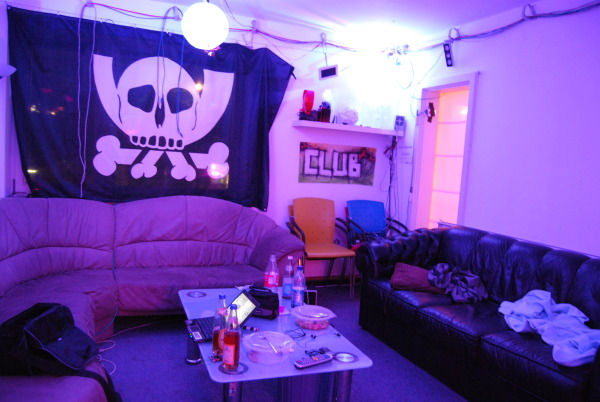
\includegraphics[width=5cm]{bilder/hbf.jpg}
%          \end{center}
%        \end{figure}

%         \begin{figure}
 %           \begin{center}
 %           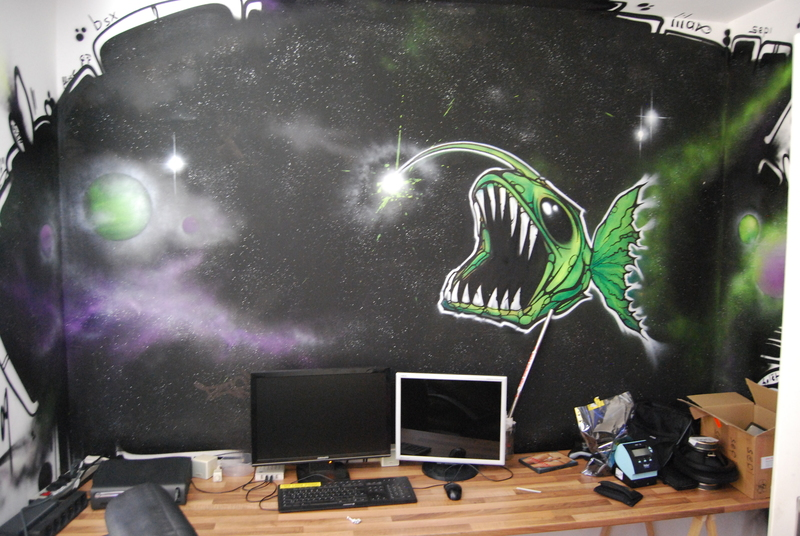
\includegraphics[width=2cm]{bilder/maxi.jpg}
 %           \end{center}
 %         \end{figure}
      \end{column}
      \begin{column}{5cm}
        \begin{figure}
          \begin{center}
          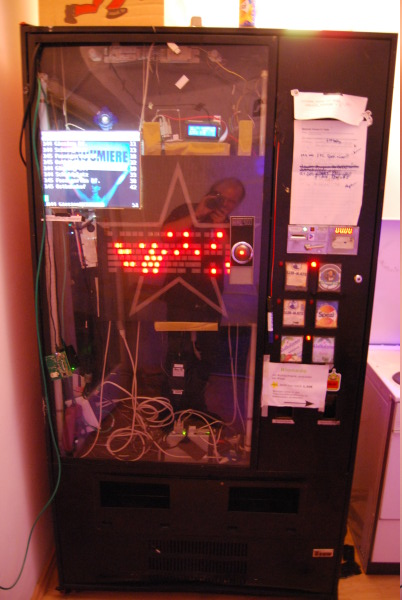
\includegraphics[width=4cm]{bilder/matemat.jpg}
%         \caption{\small matemat}
          \end{center}
        \end{figure}
%        \begin{figure}
%          \begin{center}
%          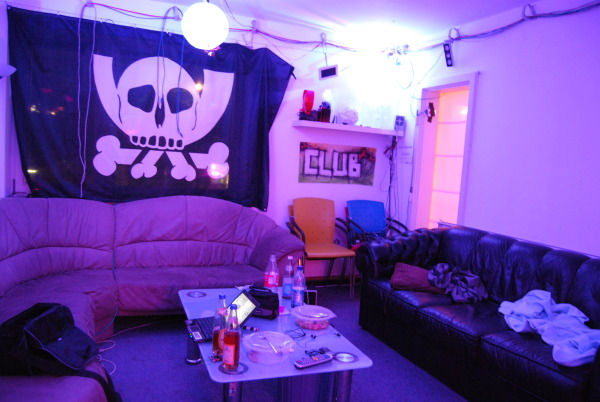
\includegraphics[width=3cm]{bilder/hbf.jpg}
%          \end{center}
%        \end{figure}
      \end{column}
    \end{columns}
    \end{frame}
\section{History}
\begin{frame}{How it came together}

\begin{columns}%[T]
\begin{column}{3.5cm}
        \begin{figure}
          \begin{center}
          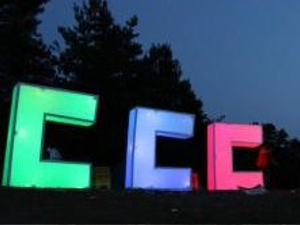
\includegraphics[width=3cm]{bilder/ddc_har.jpg}
          \caption{Moodlamp}
         % members' RGB-LED project, \\were in use for the 3c
          \end{center}
        \end{figure}
\end{column}
\begin{column}{3.5cm}
        \begin{figure}
          \begin{center}
          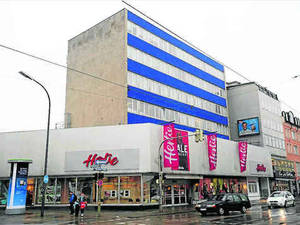
\includegraphics[width=3cm]{bilder/hertie.jpg}
          \caption{Puerto Giesing}
          %old office building,\\used by artists before beeing torn down
          \end{center}
        \end{figure}
\end{column}
\begin{column}{3.5cm}
        \begin{figure}
          \begin{center}
          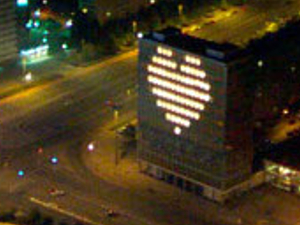
\includegraphics[width=3cm]{bilder/blinkenlights.jpg}
          \caption{Blinkenlights}
          %well known project transforming buildings into b\textbackslash w displays
          \end{center}
        \end{figure}
\end{column}
\end{columns}
\begin{columns}[T]
\begin{column}{3.5cm}
        \begin{figure}
          \begin{center}
          Members' RGB-LED project, \\were in use for the 3c
          \end{center}
        \end{figure}

\end{column}
\begin{column}{3.5cm}
        \begin{figure}
          \begin{center}
          Old office building,\\used by artists before beeing torn down
          \end{center}
        \end{figure}

\end{column}
\begin{column}{3.5cm}
        \begin{figure}
          \begin{center}
          Well known project transforming buildings into b\textbackslash w displays
          \end{center}
        \end{figure}

    \end{column}
\end{columns}
\end{frame}
\section{Hardware}
 \subsection{Development of the Lamp}
  \begin{frame}{a lamp fit for the project}
    \begin{columns}
      \begin{column}{3.5cm}
        \begin{figure}
          \begin{center}
          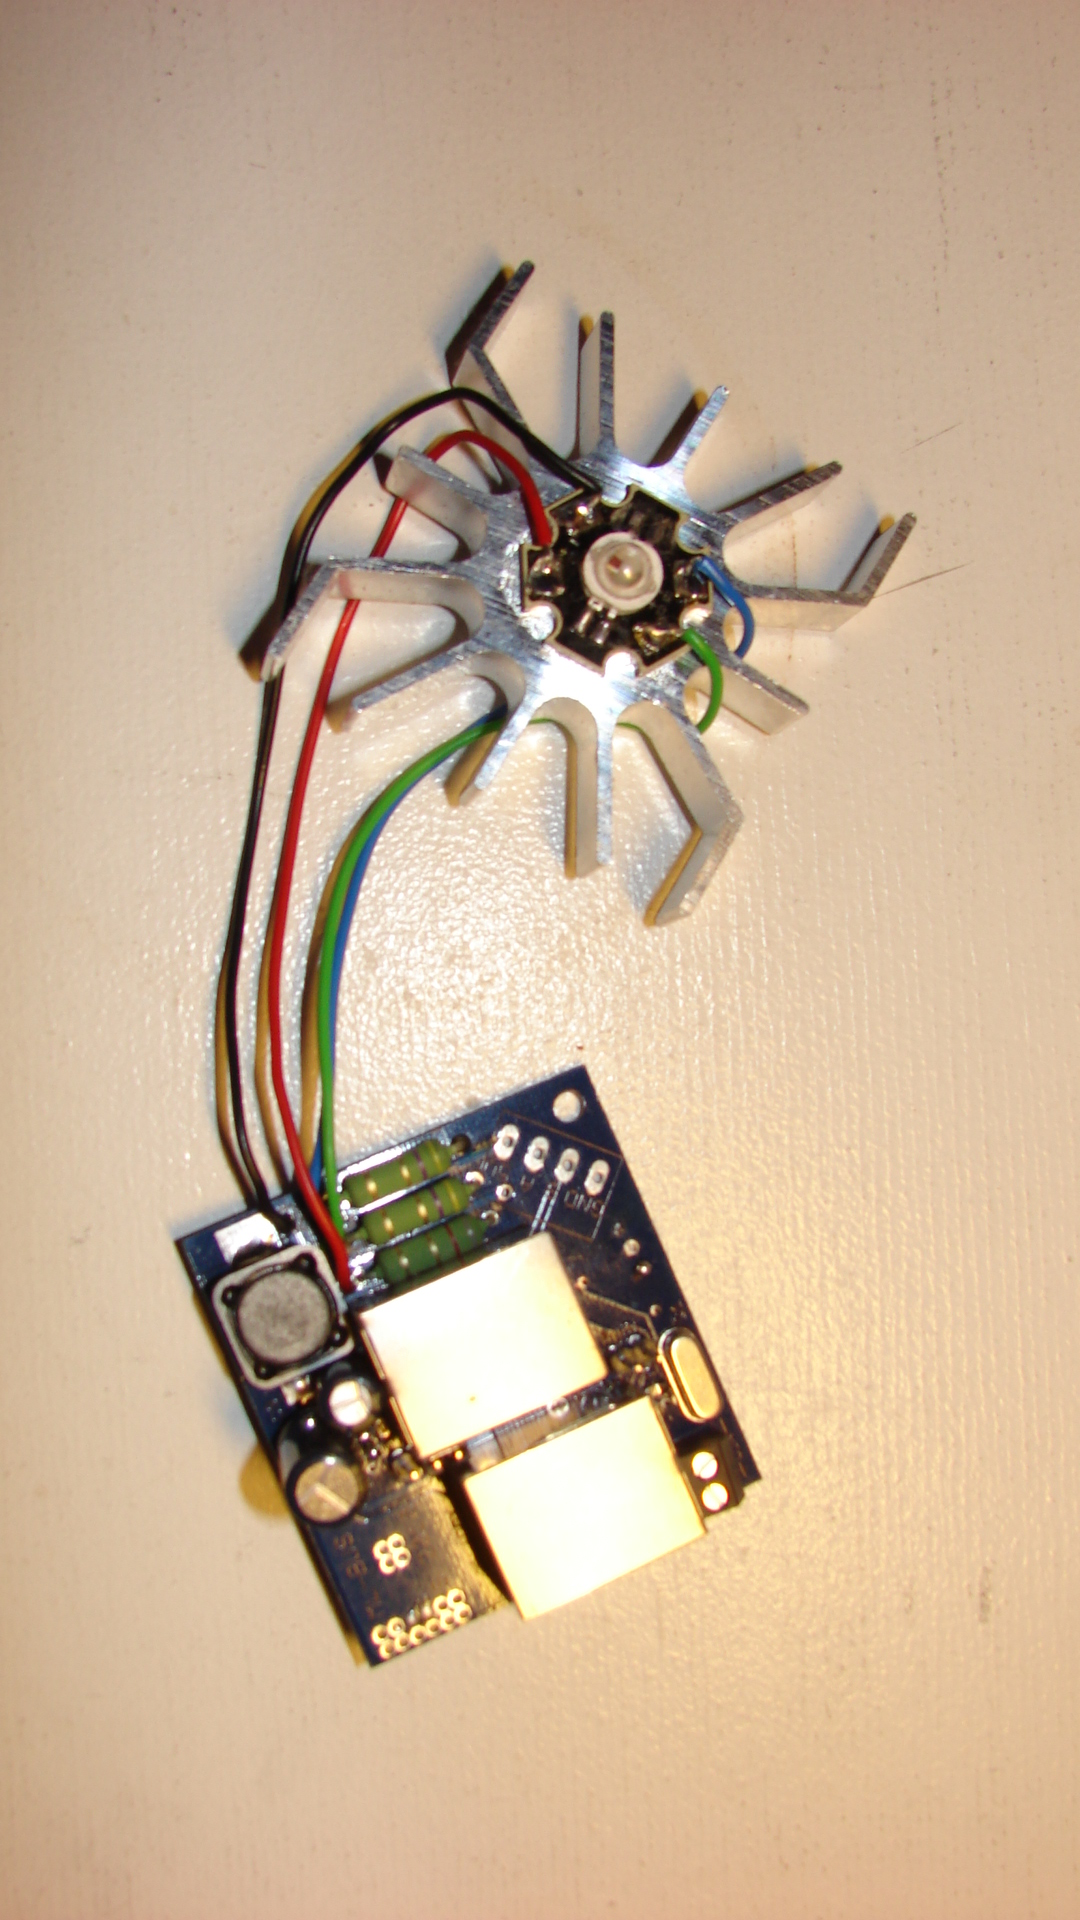
\includegraphics[width=3cm]{bilder/lampe1.JPG}
          \end{center}
        \end{figure}
      \end{column}
      \begin{column}{5cm}
        \begin{itemize}
        \item Not needed ways of communication removed (ir, usb, \ldots)
        \item Switching regulator added for higher supply voltage (-> lower supply current)
        \item Ethernet connectors replace screw terminals for faster and more stable(?) connections
        \end{itemize}
      \end{column}
      \begin{column}{3.5cm}
         \begin{figure}
          \begin{center}
          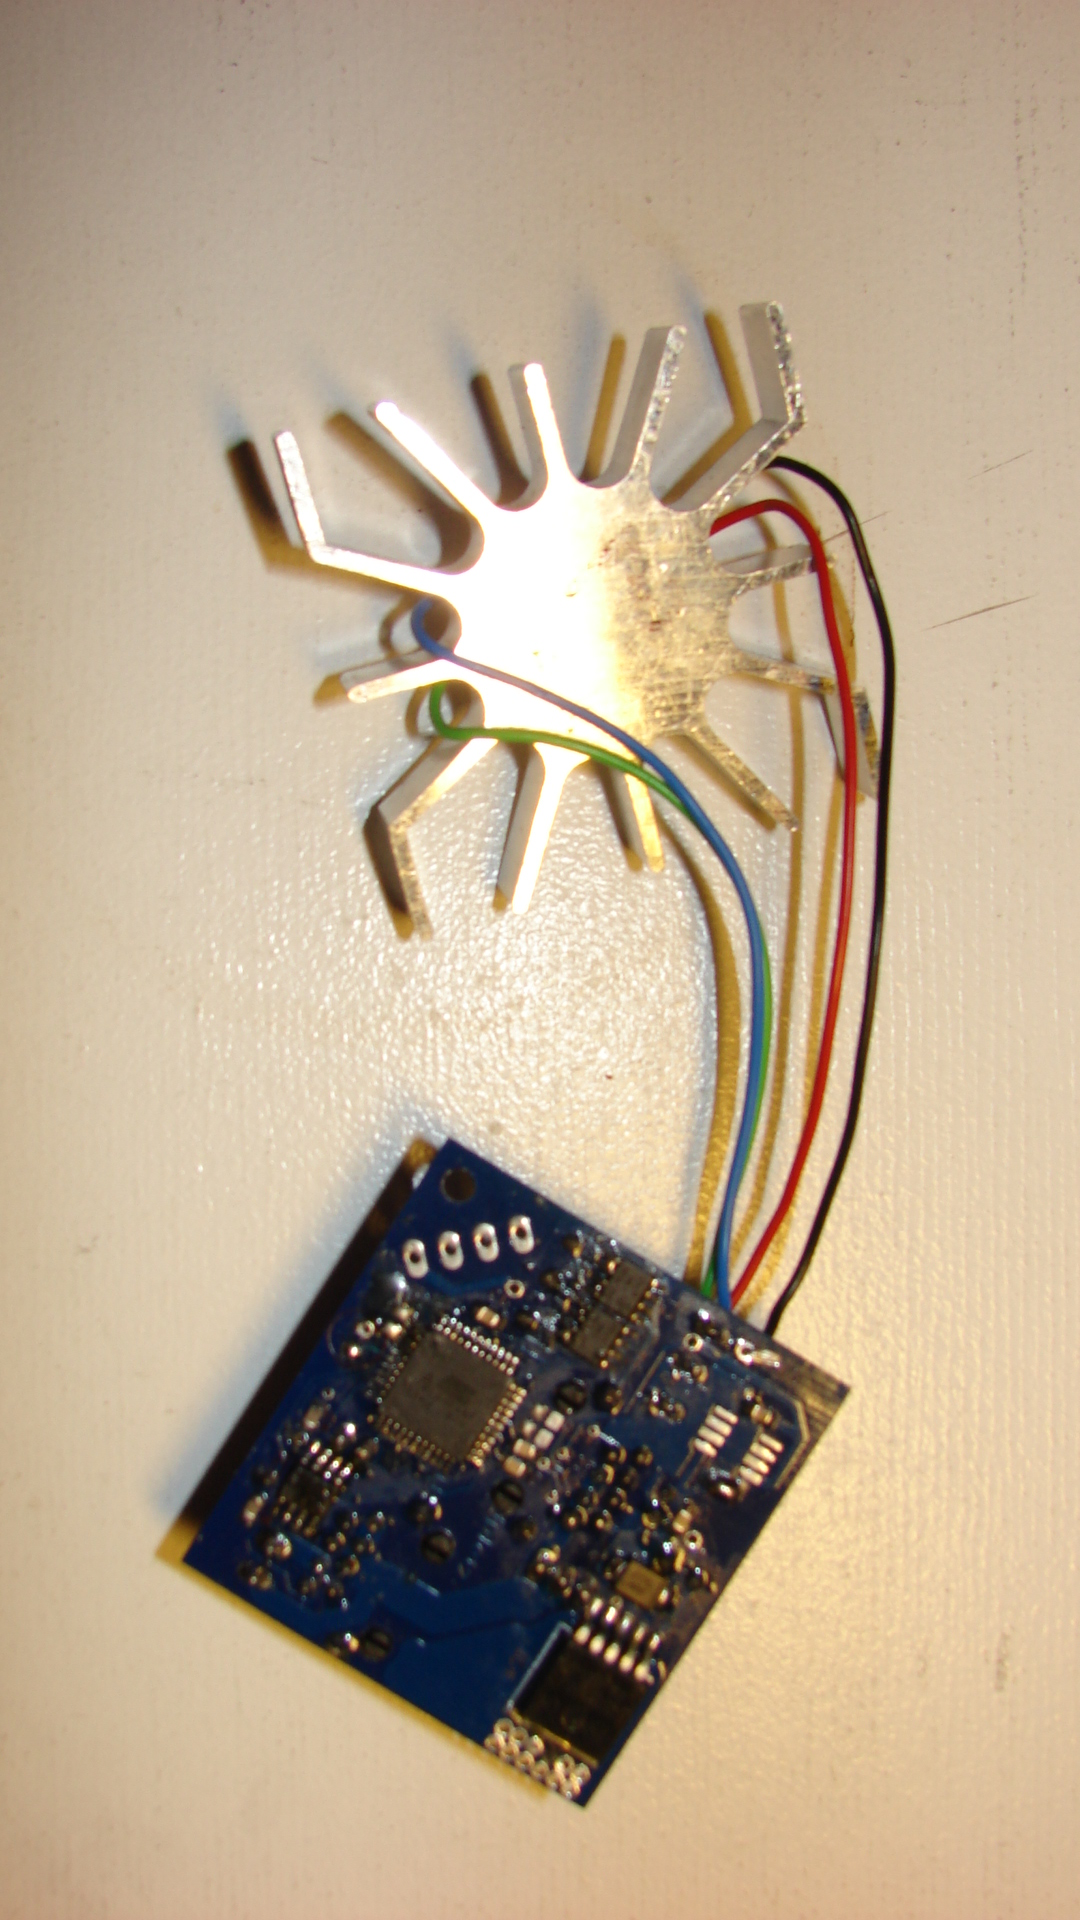
\includegraphics[width=3cm]{bilder/lampe2.JPG}
          \end{center}
        \end{figure}
     \end{column}
    \end{columns}
  \end{frame}
  \begin{frame}{The lamp - Outline}
    \begin{figure}
    \begin{center}
    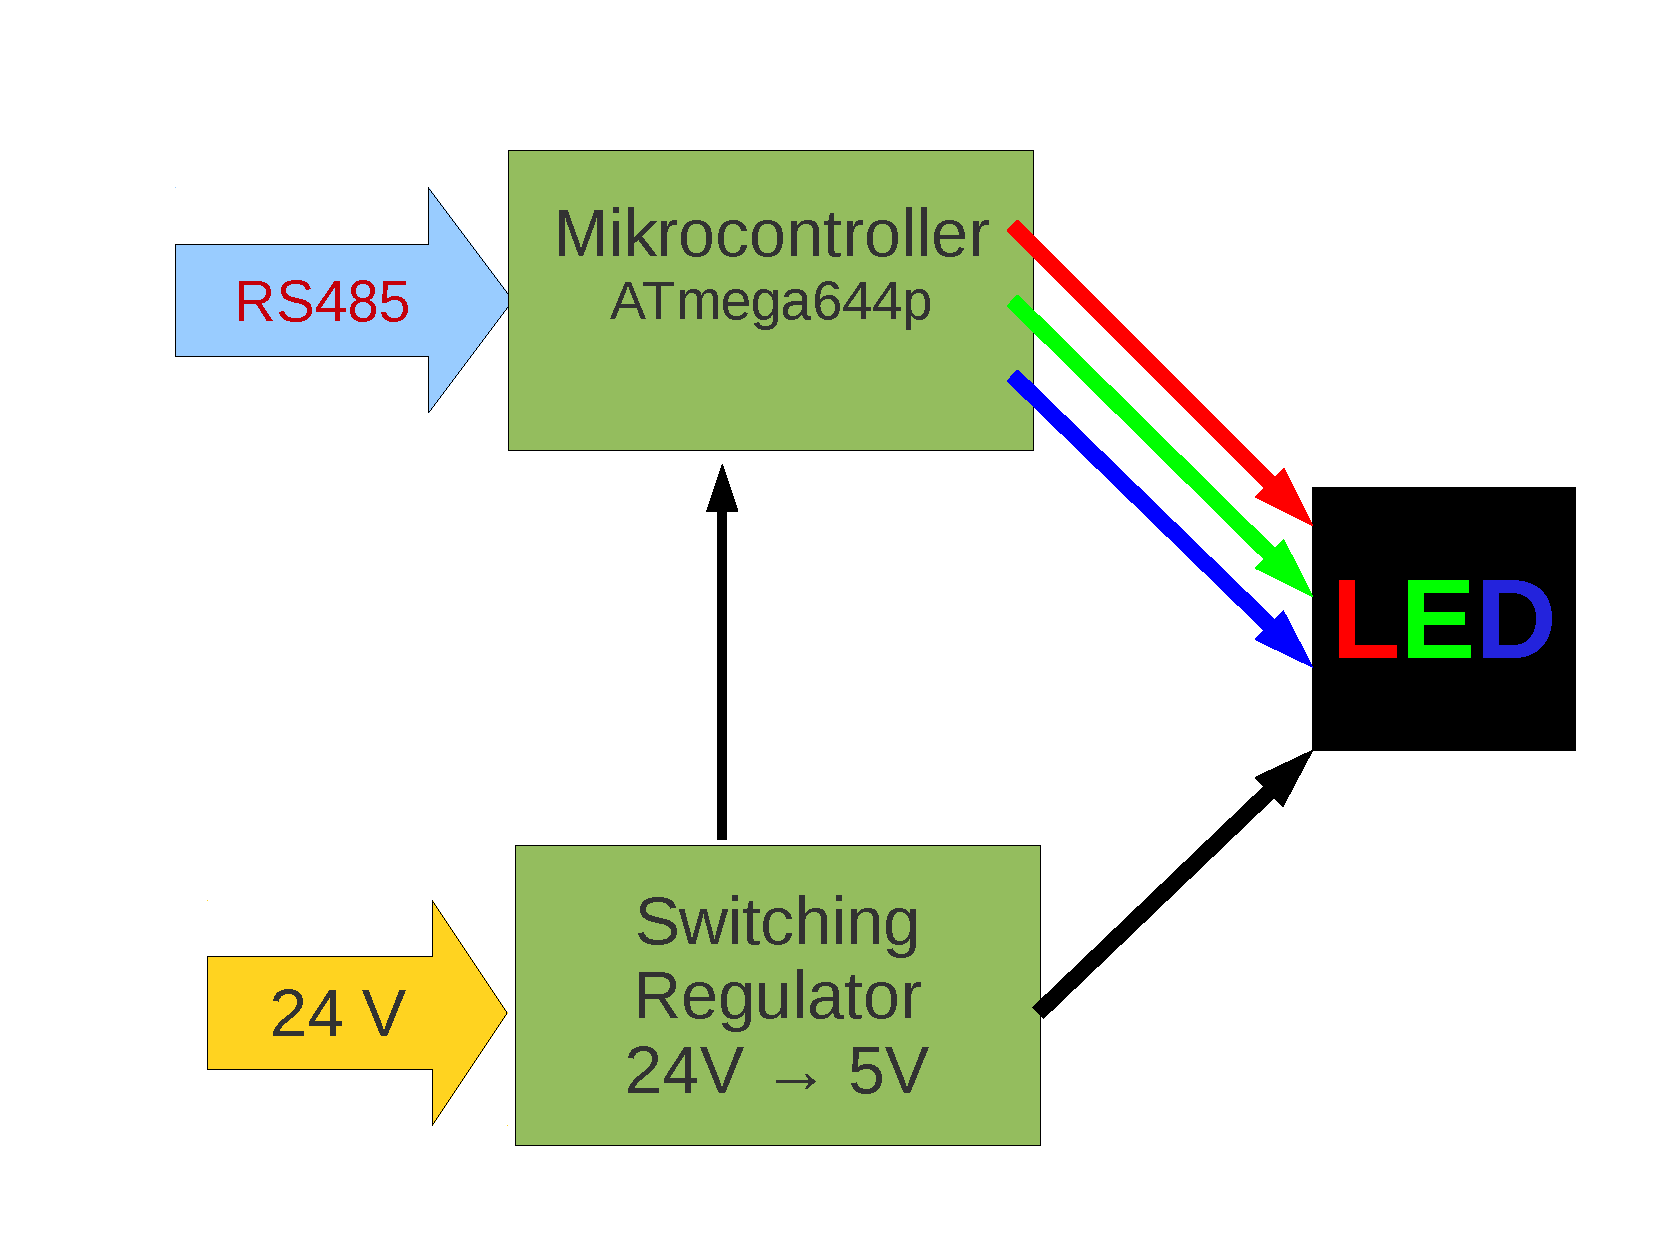
\includegraphics[width=9cm]{bilder/led_12v_rs485.pdf}
    \end{center}
    \end{figure}
  \end{frame}
\subsection{Powersupply}
  \begin{frame}{Powersupply}
  At 24V supplyvoltage the current from one power supply unit suffices for 16 lamps.
  \begin{columns}
    \begin{column}{4cm}
     \begin{block}{ Puerto Giesing}
     Two supply units are used to supply the 24 lamps of one row
     \end{block}
     \begin{block}{27c3}
     One supply unit is used for the 16 lamps of one row
     \end{block}
    \end{column}
    \begin{column}{7cm}
    \begin{figure}
    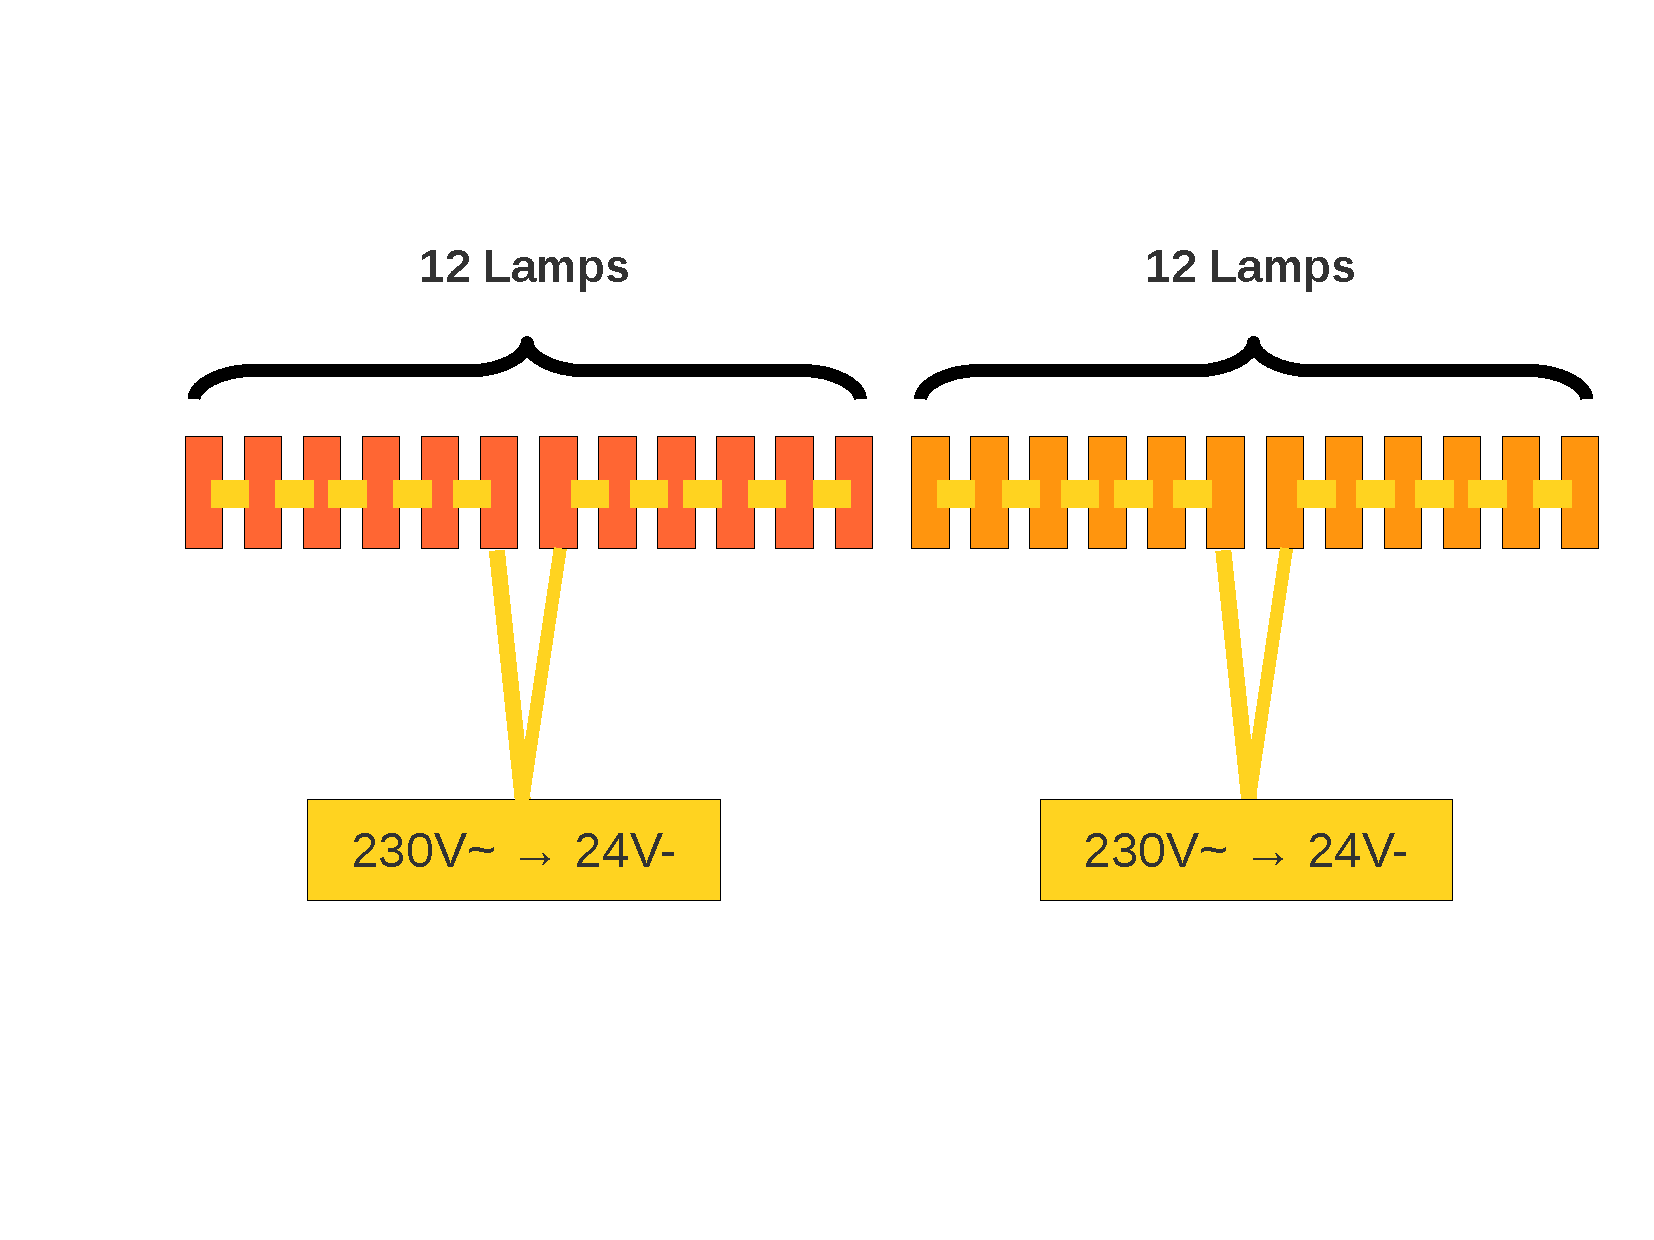
\includegraphics[width=7cm, clip, trim= 2.5cm 4.6cm 0.5cm 4cm]{bilder/12lampen.pdf}
    \end{figure}
    \end{column}
  \end{columns}
  \end{frame}
\subsection{Data Exchange}
  \begin{frame}{Data Exchange}
    \begin{itemize}
      \item Data exchange over regular ethernet cables
      \item 3 conductor pairs reserved for power supply
      \item Remaining one used for data
    \end{itemize}
      \begin{figure}
        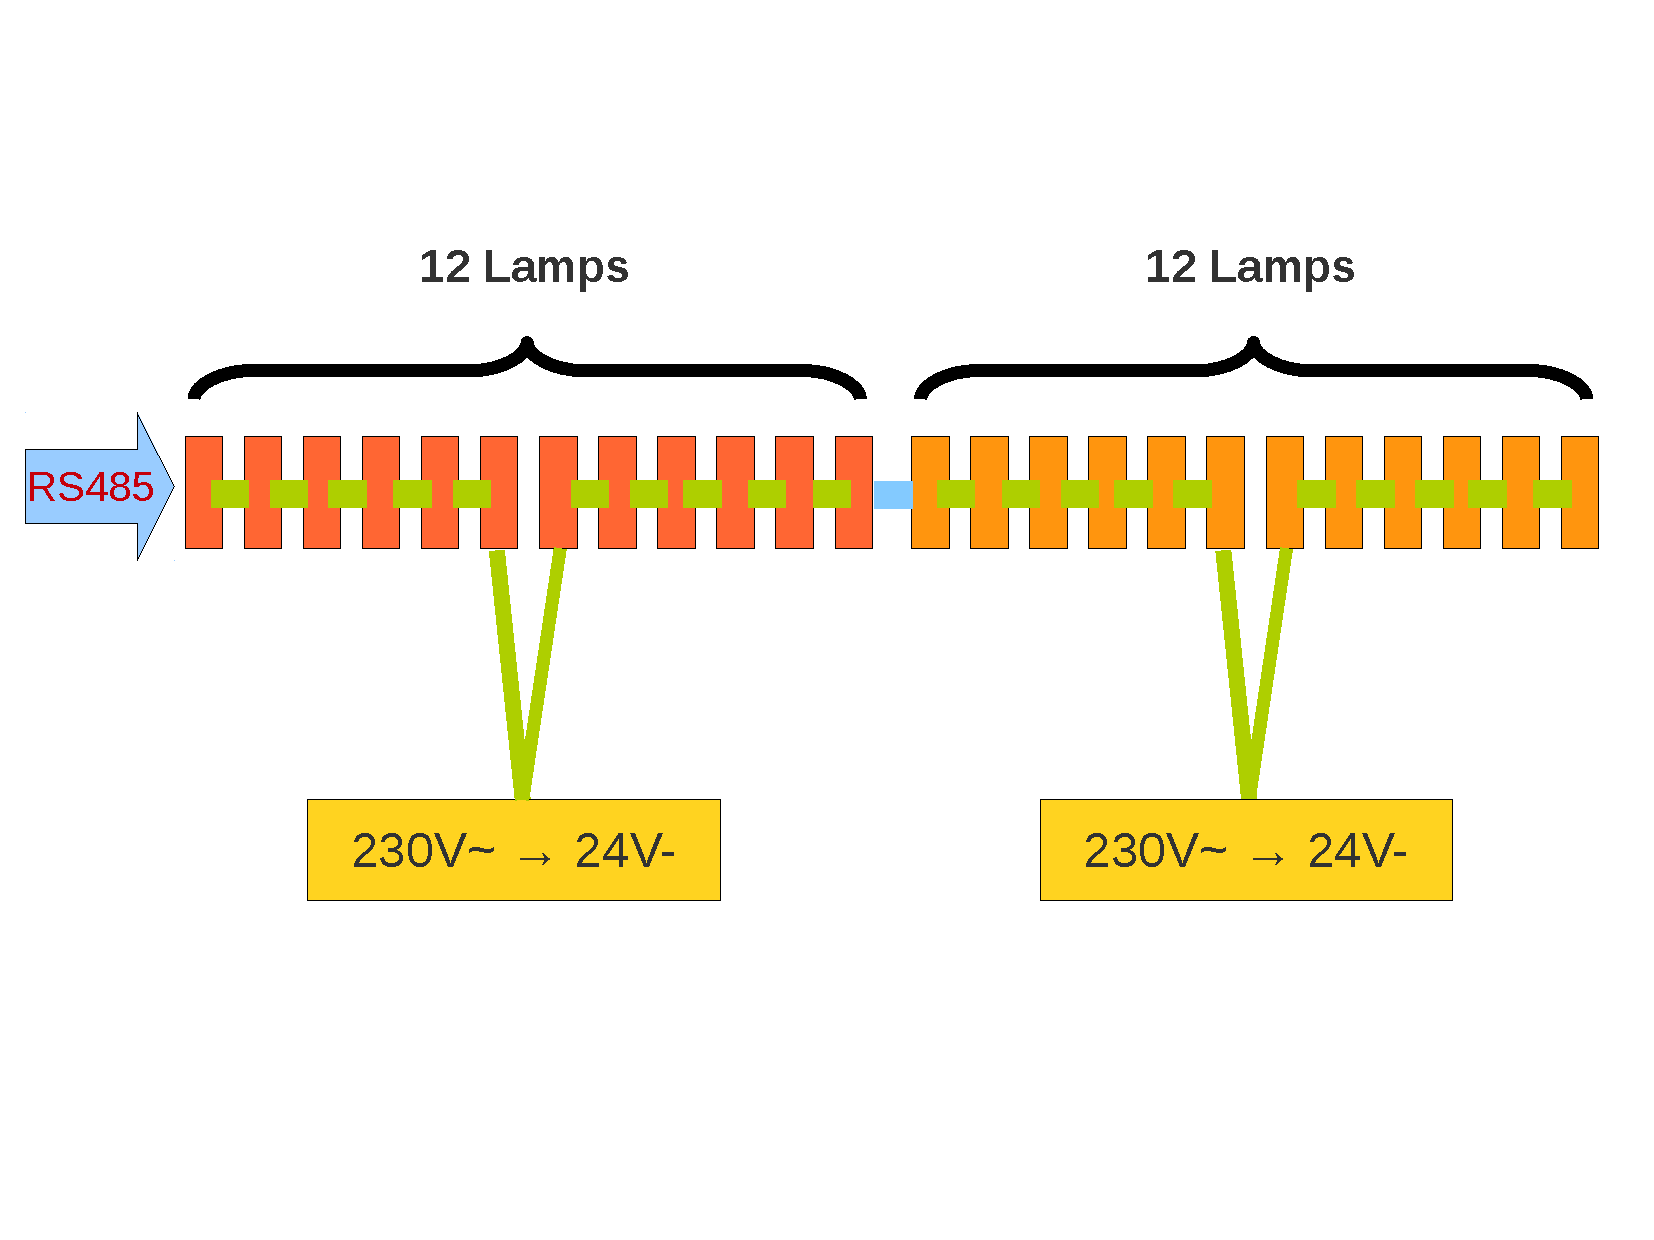
\includegraphics[width=8cm, clip, trim= 0cm 4.6cm 0.5cm 4cm]{bilder/12lampen_rs485.pdf}
        \caption{Puerto Giesing}
      \end{figure}
  \end{frame}
  \begin{frame}{RS485}
    \begin{columns}
       \begin{column}{6cm}
        \begin{figure}
        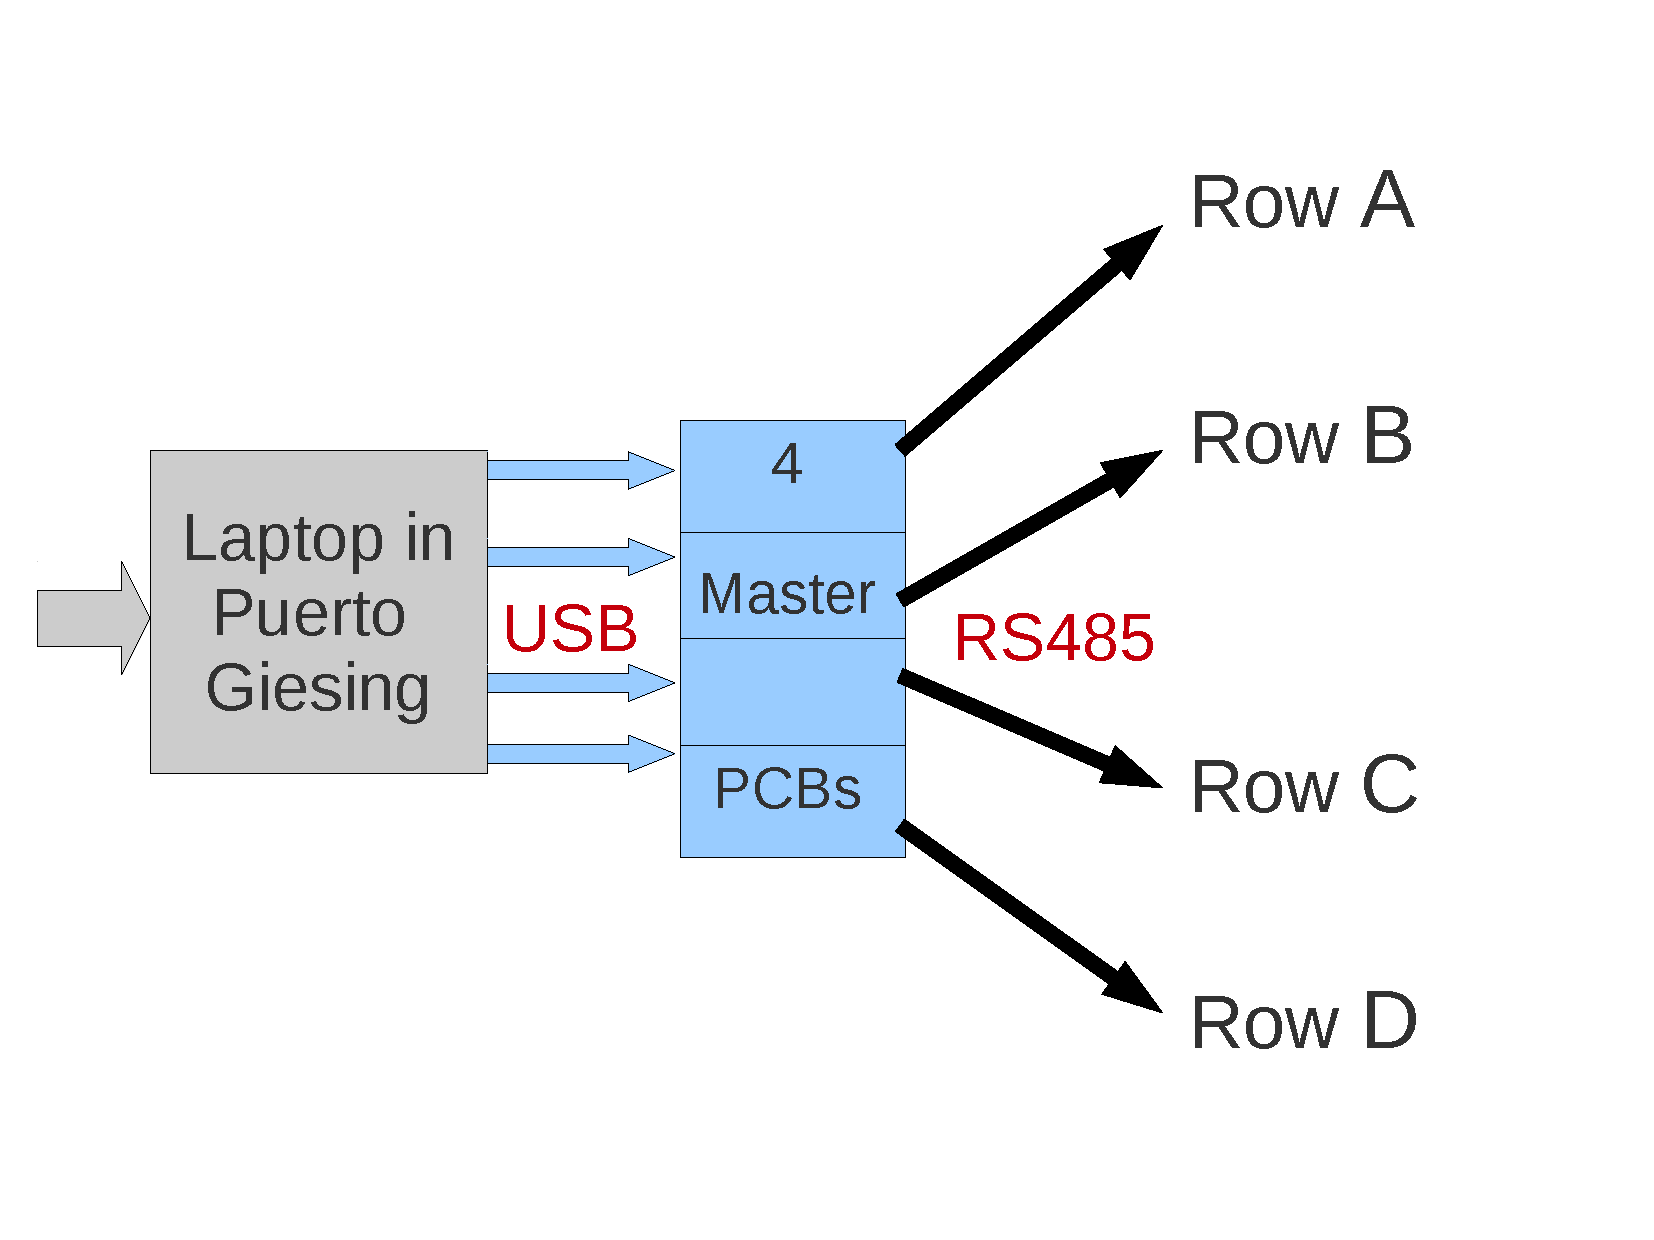
\includegraphics[width=6cm, clip, trim= 1cm 3cm 4cm 2.5cm]{bilder/laptop.pdf}
        \end{figure}
      \end{column}
      \begin{column}{5cm}
      \begin{block}{RS485}
        \begin{itemize}
        \item Versatile communication standard
        \item Connects several devices in bus structure
        \item Communication over long distances
        \end{itemize}
      \end{block}
     \end{column}
   \end{columns}
  \end{frame}

\section{Software}
\begin{frame}{Put together}
  \begin{columns}
    \begin{column}{9cm}
      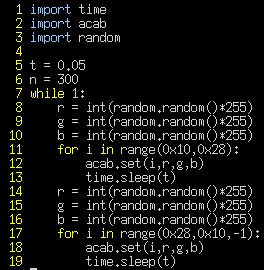
\includegraphics[width=6cm, clip, trim= 0 0 0 0]{bilder/fill.png}
% ACHTUNG aktuell falsches Bild, teil des codes fehlt
    \end{column}
  \end{columns}
\end{frame}
\section{Interaction}
    \subsection{acabed}
    \subsection{Activating Animations by sms}
    \subsection{blubbtris by dasAquarium}
\section{acab@27c3}
  \begin{frame}{acab@27c3}
    \begin{columns}
      \begin{column}{9cm}
            \begin{itemize}
               \item Plastik boxes instead of windows
               \item 6 lines with 16 boxes (text is possible)
               \item -> 6 buses, 16 lamps powered by one powersupply
               \end{itemize}
      \end{column}
   \end{columns}
  \end{frame}
\section{acab anywhere}
  \begin{frame}{acab anywhere}
  \begin{columns}
    \begin{column}{5cm}
      Software
      \begin{itemize}
      \item Mapping of lampIDs possible to any combination of lines and columns\\
      \item Fast adjustments in acabed and gigargoyle
      \end{itemize}
    \end{column}
    \begin{column}{5cm}
    Hardware
      \begin{itemize}
      \item 100 lamps available
      \item > 100 plastic boxes for versatile inside/outside installations
      \end{itemize}
    \end{column}
  \end{columns}
\vskip 0.5cm
  \begin{columns}
    \begin{cloumn}
      Finances
      \begin{itemize}
      \item start early\ldots
      \item support from the city (or other funds)
      \item private donations -> 'Pixelpaten' (godfathers for lamps)
      \end{itemize}
    \end{column}
  \end{columns}
  \end{frame}

\section{Contact}
\begin{frame}{Contact overview}
  \begin{block}{Information}
    \begin{itemize}
      \item \url{http://acab.muc.ccc.de/}
      \item \url{http://muc.ccc.de/}
      \item \url{info@muc.ccc.de}
      \item \url{presse@muc.ccc.de}
    \end{itemize}
  \end{block}
  \begin{block}{Code}
    \begin{itemize}
      \item \url{https://github.com/muccc/acabed}
      \item \url{https://github.com/muccc/gigargoyle}
    \end{itemize}
  \end{block}
\end{frame}
\end{document}
